% Figura: Criptografia nos pilares da SI
\begin{figure}[H]
    \centering
    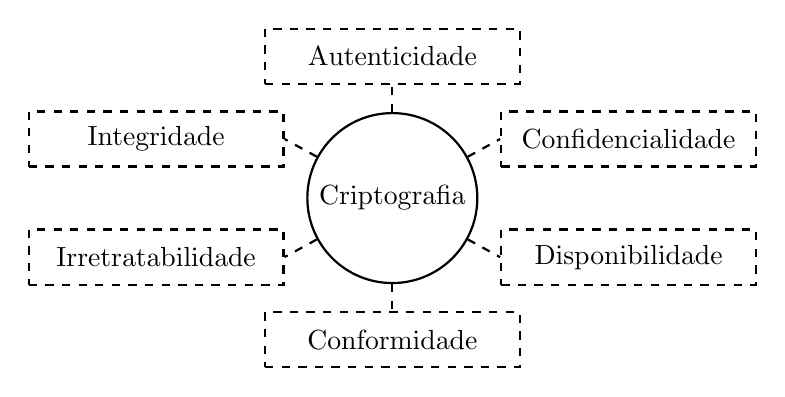
\begin{tikzpicture}
    
        % Styles
        \tikzset{dblock/.style={draw,thick,dashed,text width=3cm,minimum height=0.7cm,align=center},line/.style={-latex}};
        
        % Nodes
        \node[circle, draw, thick]         (c)  {Criptografia};
        \node[dblock, thick] at (3,0.75)   (s1) {Confidencialidade};
        \node[dblock, thick] at (-3,0.75)  (s2) {Integridade};
        \node[dblock, thick] at (3,-0.75)  (s3) {Disponibilidade};
        \node[dblock, thick] at (-3,-0.75) (s4) {Irretratabilidade};
        \node[dblock, thick] at (0, 1.8)   (s5) {Autenticidade};
        \node[dblock, thick] at (0, -1.8)  (s6) {Conformidade};
        
        % Arrows
        \draw[-, thick, dashed] (c) to (s1.west);
        \draw[-, thick, dashed] (c) to (s2.east);
        \draw[-, thick, dashed] (c) to (s3.west);
        \draw[-, thick, dashed] (c) to (s4.east);
        \draw[-, thick, dashed] (c) to (s5.south);
        \draw[-, thick, dashed] (c) to (s6.north);
    
    \end{tikzpicture}
    \caption{Criptografia apoiada nos pilares da SI.}
    \label{fig:criptografiaSI}
\end{figure}